% !TEX root = ../main.tex
\section{Background}
\label{sec:background}

Section~\ref{sec:related-work-gap} ended with a gap: none of the reviewed studies
compares two explainability methods on the same crops as a function of a controlled
object-to-image (O2I) ratio, against a complex industrial background, with a per-pixel
measure of whether the evidence lies on the object or on the background. The concepts
needed to close it follow the order of the experiment, namely the data
(Section~\ref{sec:background-dataset}), the controlled variable
(Section~\ref{sec:background-o2i}), the classifier and its training
(Sections~\ref{sec:background-cnn} and~\ref{sec:background-training}), the two
explainability methods (Sections~\ref{sec:background-occlusion}
and~\ref{sec:background-gradcam}) and the measure that compares them
(Section~\ref{sec:background-comparison}).

% ============================================================================
\subsection{The Learning Factory Dataset}
\label{sec:background-dataset}

\paragraph{The learning factory}
All images in this thesis show the Fischertechnik Industry~4.0 learning factory, a
model production line with five modules, namely a sorting machine, an oven, a milling
machine, a high-bay warehouse and a vacuum gripper~\cite{schneidereitFischertechnik2023,
schneidereitYOLOv8}. Fig.~\ref{fig:bg-dataset}\,(a) shows one photograph of it. Around a
workpiece, the photographs contain red and blue building blocks, many black parts,
cables and the grey base plate. This is the complex background that both earlier
studies on the learning factory examined.

\paragraph{Workpieces and capture protocol}
The dataset was created by T.~Schneidereit, Gohrenz and
Breu{\ss}~\cite{schneidereitYOLOv8}. It contains 15 cylindrical workpieces that differ in
material and colour and fall into four families: six plastics (white, red, blue,
yellow, grey and black), four workpieces of acrylic glass (AG; orange, yellow, blue and
red), three metals (aluminium, brass and steel) and two woods (light and dark). The plastic
workpieces are 3D printed from PETG, the acrylic glass is fluorescent, and the plastic,
AG and metal workpieces match the dimensions of the default workpieces of the learning
factory, while the wooden ones are knothole dowels. Each
workpiece was photographed at the same 33 positions in each of the five modules, or
stations, which gives 165 photographs per workpiece and 2,475 in
total.\footnote{The copy of the dataset used in this thesis holds 166 photographs per
material, 2,490 in total, with 33 at each of the stations one to four and 34 at station
five. All 166 are used.} Between recordings, the lighting was varied and the camera
position was changed, so the workpieces were photographed from different angles and
distances. At a given position, viewpoint and lighting are the same for all 15
workpieces. Within one material, the background and the viewpoint therefore change from
photograph to photograph, while across materials at one position, by design, only the
workpiece changes.

\paragraph{Labels}
Each photograph has $960 \times 720$ pixels and was labelled with labelImg in the format
of the YOLO (You Only Look Once) detector~\cite{redmon2016yolo}. A label file holds one
line per object, and every photograph of this dataset contains exactly one workpiece.
The line consists of a class index and four numbers, the box centre $(x_c, y_c)$, the
width $w$ and the height $h$, each divided by the width or height of the photograph so
that they lie in $[0,1]$. Fig.~\ref{fig:bg-dataset}\,(b) marks these quantities for
photograph 2024-04-15-095336, a photograph of black plastic from the validation split
that serves as the real example throughout this chapter. Its box measures
$36 \times 33$ pixels, i.e., about 0.17\% of the photograph, and is smaller than the
median box over all 2,490 labels, $50 \times 46$ pixels or 0.33\%. On the whole
photograph, the workpiece is thus a small object by the 1\% criterion collected by
Nikouei et al.~\cite{nikouei2025smallobject} (Section~\ref{sec:related-work-industrial}).
The box, however, tells where the workpiece is, and that makes it possible to cut crops
in which it covers a prescribed part of the image. During the exploration of the dataset,
two label files with a class index outside the range 0 to 14 were found in the folder
that holds all photographs together. They were reported to the dataset authors and
corrected; the labels used here were not affected.

\begin{figure}[tbp]
\centering
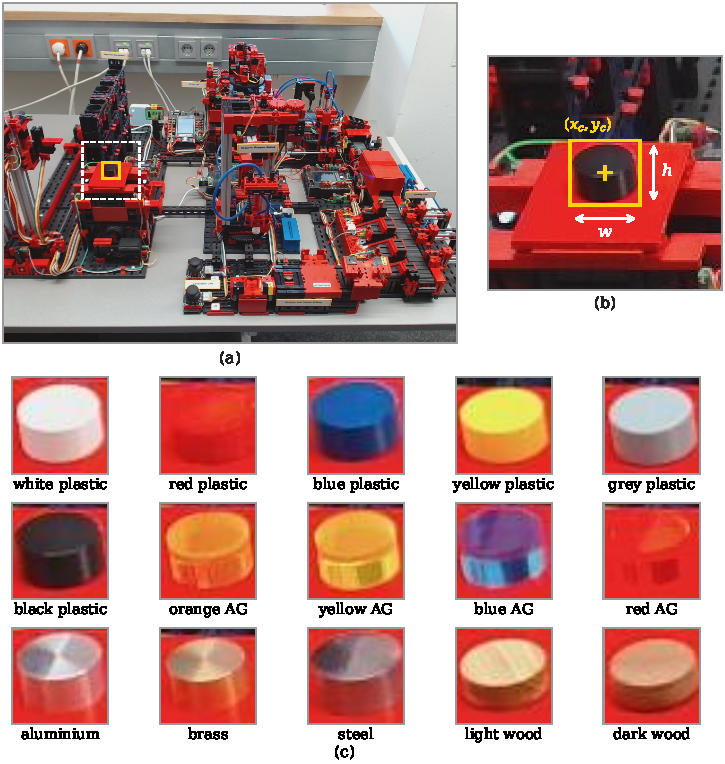
\includegraphics[width=\textwidth]{ch3_figures/fig_ch3_dataset.pdf}
\caption[Learning factory and the 15 workpieces]{Fischertechnik Industry~4.0 learning
factory and the 15 workpieces, where AG is an abbreviation for acrylic glass.
(a) Photograph 2024-04-15-095336 ($960 \times 720$ pixels) with the bounding box of the
black plastic workpiece (yellow) and the enlarged region (white, dashed); (b) enlarged
region with the box centre $(x_c, y_c)$, width $w$ and height $h$ of the label in the
format of the YOLO (You Only Look Once) detector; (c) the 15 workpieces at the same
position, cropped at an object-to-image (O2I) ratio of 90\%. Source of the photographs:
dataset of \cite{schneidereitYOLOv8}.}
\label{fig:bg-dataset}
\end{figure}

\paragraph{Why this dataset}
Four properties make the dataset suitable for the research question. The background
shares colours with several workpieces. Both earlier studies traced detection errors to
such an overlap, the 2023 study for the red workpieces and the 2025 study, with a hedge,
for black plastic among the many black parts of the learning factory
(Section~\ref{sec:related-work-fischertechnik}). Fig.~\ref{fig:bg-dataset}\,(c) shows
the overlap at a single position. Red plastic and red AG almost disappear against the
red plate on which they lie there, and aluminium, steel and grey plastic look much
alike, a similarity that the 2025 study also points out. Aluminium also occurs in the
learning factory itself, which uses it for the supports of the suction
pads~\cite{schneidereitYOLOv8}. These similarities are intended: the 2025 study chose
several workpieces for them, e.g., the black workpiece because it matches the many black
parts of the learning factory. For black plastic, the
workpiece of the real example, the overlap is with the dark parts of the learning
factory rather than with the plate. Since every material was photographed at the same
positions, the models of different materials see the same scenes, and a difference
between them cannot come from a different set of backgrounds. The single box per
photograph allows a crop with a prescribed share of workpiece, which is the variable of
the experiment. Finally, the per-material results of the 2025 study give a reference
point for the material ranking found here, although task and metric differ
(Section~\ref{sec:related-work-fischertechnik}).

\paragraph{Limitation}
Each material is represented by one physical workpiece that was photographed 166 times.
A model can therefore learn properties of that particular piece, e.g., a scratch or the
grain pattern of one piece of wood, together with properties of its material, and the
data cannot separate the two. The results of this thesis describe these 15 workpieces.
Whether they carry over to other workpieces of the same materials is not tested.

% ============================================================================
\subsection{The Object-to-Image Ratio}
\label{sec:background-o2i}

Pawlowski et al.~\cite{pawlowski2019needles} define the O2I ratio by area,

\begin{equation}
r = 100 \cdot \frac{A_{\mathrm{obj}}}{A_{\mathrm{img}}},
\label{eq:bg-o2i}
\end{equation}

where $A_{\mathrm{obj}}$ is the area of the object and $A_{\mathrm{img}}$ the area of
the image, both in pixels, and $r$ is the ratio in percent. This thesis uses the same
definition, with a square crop centred on the box as the image and the area of the
bounding box as the object area. The box also encloses some background around the
cylindrical workpiece, so the workpiece itself covers somewhat less of the crop than
$r$ states. The crop equations and the rule for crops that would extend beyond the
photograph are given in Section~\ref{sec:methodology-crops}.

\paragraph{Area and side length}
Because the ratio is defined by area, it does not fall in proportion to the width of the
object. For a square object of side $s_{\mathrm{obj}}$ in a square image of side
$s_{\mathrm{img}}$, Eq.~\eqref{eq:bg-o2i} gives

\begin{equation}
\frac{s_{\mathrm{obj}}}{s_{\mathrm{img}}} = \sqrt{\frac{r}{100}},
\label{eq:bg-side-fraction}
\end{equation}

where both sides are in pixels and the side fraction on the left is dimensionless. For
the five ratios of this thesis, 90, 70, 50, 30 and 10\%,
Eq.~\eqref{eq:bg-side-fraction} gives 0.95, 0.84, 0.71, 0.55 and 0.32. At 10\%, a square
with the area of the box thus still spans almost a third of the crop width.

\paragraph{A toy scene}
One toy example is used throughout this chapter, small enough that every number can be
checked by hand. Its scene is a grid of $16 \times 16$ grey levels between 0 (black) and
1 (white), shown in Fig.~\ref{fig:bg-o2i}\,(a). A light background of 0.9 stands for the
learning factory, a dark $4 \times 4$ workpiece of 0.1 in the centre stands for black
plastic, and eight dark $2 \times 2$ factory parts of 0.1 are scattered over the
background. Two crops are cut from the same scene. The tight crop is the central
$8 \times 8$ region (Fig.~\ref{fig:bg-o2i}\,(b)). The workpiece covers 16 of its 64
pixels, a ratio of 25\%, and two of the factory parts fall inside it, at the top-left and
bottom-right corners. Since the toy network takes $8 \times 8$ inputs, the tight crop
needs no resizing. The loose crop is the whole scene, in which the workpiece covers
$16/256 = 6.25\%$. It is resized to $8 \times 8$ by averaging blocks of $2 \times 2$
pixels (Fig.~\ref{fig:bg-o2i}\,(c)). The workpiece then occupies $2 \times 2$ pixels,
still $4/64 = 6.25\%$, and every factory part becomes a single pixel. Resizing leaves the
ratio unchanged, but the workpiece has lost half of its width in pixels.

\paragraph{The real crops}
Fig.~\ref{fig:bg-o2i}\,(d) shows the same construction on photograph
2024-04-15-095336. The native crop sides are 36, 42, 48, 62 and 108 pixels at the five
ratios, and every crop is resized to $256 \times 256$ pixels. This photograph is
therefore enlarged about 7 times at 90\% and about 2.4 times at 10\%. At 90\% and 70\%, the crop shows almost only the
workpiece, with a thin strip of red plate and a dark band along the top edge. At 10\%,
the workpiece sits on the red plate of the module, surrounded by red building blocks, a
cable and dark structure.

\begin{figure}[tbp]
\centering
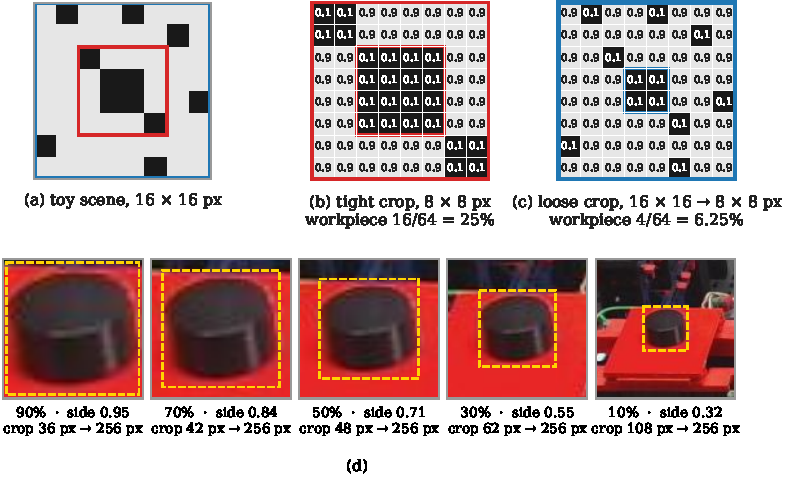
\includegraphics[width=\textwidth]{ch3_figures/fig_ch3_o2i.pdf}
\caption[Object-to-image ratio on the toy scene and on a real photograph]{Object-to-image
(O2I) ratio. (a) Toy scene of $16 \times 16$ pixels with a dark workpiece and dark
factory parts, (red) tight crop, (blue) loose crop; (b) tight crop, $8 \times 8$ pixels;
(c) loose crop, averaged in $2 \times 2$ blocks to $8 \times 8$ pixels; (d) crops of
photograph 2024-04-15-095336 at the five O2I ratios, each resized to $256 \times 256$
pixels, with (dashed) the centred square that has the area of the bounding box, and
below each crop the side fraction $\sqrt{r/100}$ and the native crop side.}
\label{fig:bg-o2i}
\end{figure}

\paragraph{What follows for the thesis}
With a fixed input size, loosening a crop changes two things together. The share of
background in the input grows, and the workpiece covers fewer input pixels. In the toy,
the workpiece shrinks from $4 \times 4$ to $2 \times 2$ pixels. In the real crops, the
side of the square with the area of the box shrinks from about 243 pixels at 90\% to
about 81 pixels at 10\% of the $256$-pixel input. Section~\ref{sec:related-work-o2i}
made this point in contrast to the digit data of Pawlowski et al., who keep the digits
at their native size, and Fig.~\ref{fig:bg-o2i} shows it directly. An effect of the ratio in this thesis
is therefore the combined effect of more background and a smaller workpiece, and the
network of Section~\ref{sec:background-cnn} shows why the second part matters.

% ============================================================================
\subsection{Convolutional Neural Networks}
\label{sec:background-cnn}

Fig.~\ref{fig:bg-cnn-toy} follows the tight toy crop through the first stages of a
convolutional neural network (CNN). A CNN computes a stack of feature maps, each from
the maps before it, and ends in a small number of scores, one per
class~\textbf{[CITATION NEEDED]}.

\paragraph{Convolution}
Let $X \in \mathbb{R}^{C \times N \times N}$ be an input with $C$ channels, e.g., the
three colour channels of a crop or the single grey channel of the toy. A convolutional
layer with $K$ kernels of size $3 \times 3$ computes

\begin{equation}
Y^k_{uv} = b^k + \sum_{q=1}^{C} \sum_{\Delta u=-1}^{1} \sum_{\Delta v=-1}^{1}
W^k_{q,\Delta u,\Delta v}\, X_{q,\,u+\Delta u,\,v+\Delta v}, \qquad k = 1, \dots, K,
\label{eq:bg-conv}
\end{equation}

where $W^k \in \mathbb{R}^{C \times 3 \times 3}$ is the $k$-th kernel with entries
$W^k_{q,\Delta u,\Delta v}$ for the offsets $\Delta u, \Delta v \in \{-1, 0, 1\}$,
$b^k \in \mathbb{R}$ its bias, $(u, v)$ the row and column of an output position, and
$Y^k \in \mathbb{R}^{N \times N}$ the output for kernel $k$. The same kernel is applied at
every position, so a pattern is detected wherever it occurs. Strictly,
Eq.~\eqref{eq:bg-conv} is a cross-correlation, since the kernel is not flipped, but
deep learning calls it a convolution~\textbf{[CITATION NEEDED]}. At the border, the sum
reaches beyond the input. Padding with one row and column of zeros on each side keeps
the output at $N \times N$, which is what the network of this thesis does. The toy
instead repeats the edge pixels, because a border of zeros would look dark to a
detector of dark regions.

The toy network has two kernels. The dark detector has all nine weights equal to $-1/9$
and the bias $+0.6$ (Fig.~\ref{fig:bg-cnn-toy}\,(b)), so its output is 0.6 minus the
mean of the $3 \times 3$ neighbourhood, positive wherever that mean is below 0.6. On the
inside of the workpiece it gives $0.6 - 0.1 = 0.50$, and on open background
$0.6 - 0.9 = -0.30$ (Fig.~\ref{fig:bg-cnn-toy}\,(c)). The light detector has the
weights $+1/9$ and the bias $-0.7$ and responds where the mean is above 0.7.

\paragraph{Rectified linear unit}
The rectified linear unit (ReLU) keeps positive values and sets negative ones to zero,
$A^k = \max(Y^k, 0)$ element by element~\textbf{[CITATION NEEDED]}. The result
$A^k \in \mathbb{R}_{\ge 0}^{N \times N}$ is the feature map of channel $k$.
Fig.~\ref{fig:bg-cnn-toy}\,(d) shows the dark feature map $A^1$ of the tight crop. The
dark detector responds to any dark region that fills its $3 \times 3$ neighbourhood,
whether it belongs to the workpiece or not. Here this is the case at both factory parts,
whose neighbourhoods at the corners of the crop are completed by the repeated border,
and they reach the same 0.50 as the centre of the workpiece. The feature map says where
something dark is, not whether it belongs to the workpiece. This is the situation of
black plastic among the many black parts of the learning factory, with which the 2025
study, with a hedge, explained the difficulty of its detector with this workpiece
(Section~\ref{sec:related-work-fischertechnik}).

\paragraph{Max pooling}
Max pooling with $2 \times 2$ windows halves the resolution by keeping the largest value
of each window~\textbf{[CITATION NEEDED]},

\begin{equation}
M^k_{uv} = \max_{\Delta u,\,\Delta v \in \{0, 1\}} A^k_{2u+\Delta u,\,2v+\Delta v},
\label{eq:bg-maxpool}
\end{equation}

where $M^k \in \mathbb{R}_{\ge 0}^{N/2 \times N/2}$ is the pooled map and $(u, v)$ now
indexes the windows. A response survives pooling if it is the strongest in its window,
and its exact position inside the window is lost. Where several cells of a window share
the maximum, the maximum is not differentiable, and the implementation passes the
gradient to one of them. In the toy, the pooled dark map of
Fig.~\ref{fig:bg-cnn-toy}\,(e) has $4 \times 4$ cells, with 0.50 in the four cells of the
workpiece and in the two corner cells of the factory parts.

\paragraph{From feature maps to a decision}
After the last convolution, the feature maps are summarised into a vector of fixed
length. Adaptive average pooling divides each map into a fixed grid of regions, here
$4 \times 4$, and averages each region. A fully connected layer then computes each of
its outputs as a weighted sum of all its inputs plus a bias. The last layer returns the
logits, real-valued scores without bounds, one per class, which the softmax of
Section~\ref{sec:background-training} turns into probabilities. The toy network instead
takes the mean of each whole pooled map, the special case with a single region, called
global average pooling~\textbf{[CITATION NEEDED]}. This gives
$g = (g_1, g_2) = (0.201, 0.125)$ for the dark and the light channel. A single linear
unit with the weights $(10, -5)$ and no bias then returns the logit
$z = 10 \cdot 0.201 - 5 \cdot 0.125 = 1.39$, and a positive $z$ stands for the decision
``black plastic''. The toy network thus rewards dark regions and penalises light
ones.

\paragraph{Receptive field}
Each value of a feature map depends only on a limited region of the input, its receptive
field~\textbf{[CITATION NEEDED]}. In the toy, one value of $A^1$ sees $3 \times 3$
pixels. Through the four
convolutional layers of the network of this thesis and the three poolings between them,
its width grows as $1 \to 3 \to 4 \to 8 \to 10 \to 18 \to 22 \to 38$ pixels, and the
derivation is given in Section~\ref{sec:methodology-patch}. A unit of the fourth
convolutional layer therefore sees $38 \times 38$ input pixels. The square with the area
of the box spans about 6.4 such widths at 90\% and about 2.1 at 10\%. A pattern detector
of fixed size thus meets a smaller workpiece in a looser crop.

Fig.~\ref{fig:bg-cnn-toy}\,(f) shows what this does to the toy. In the loose crop, the
workpiece covers $2 \times 2$ pixels and no longer fills a $3 \times 3$ neighbourhood.
The dark detector gives only 0.06 on the workpiece itself, and at most 0.14 where a
factory part, now a single pixel, lies diagonally next to it, instead of 0.50 in the
tight crop. The global averages become $g = (0.025, 0.100)$, and the logit falls from
1.39 to $-0.25$. The toy network fails at the small ratio, although the workpiece has not changed. The
toy was built to make this visible, and how strongly the real network is affected cannot
be read from it. It is, however, the scale effect that Section~\ref{sec:methodology-covariates} lists among the
quantities that change together with the ratio.

\begin{figure}[tbp]
\centering
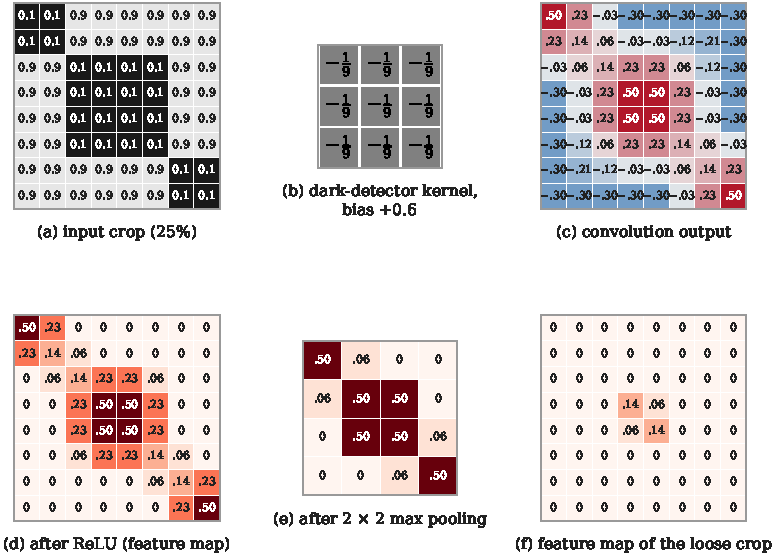
\includegraphics[width=\textwidth]{ch3_figures/fig_ch3_cnn_toy.pdf}
\caption[Building blocks of a CNN on the toy crop]{Building blocks of a convolutional
neural network (CNN) on the toy crop. (a) Grey levels of the tight crop;
(b) $3 \times 3$ kernel of the dark detector, bias $+0.6$; (c) convolution output,
(blue) negative, (red) positive; (d) feature map after the rectified linear unit (ReLU);
(e) after $2 \times 2$ max pooling; (f) feature map of the loose crop of
Fig.~\ref{fig:bg-o2i}\,(c), on the same colour scale as (d).}
\label{fig:bg-cnn-toy}
\end{figure}

\paragraph{The network of this thesis}
All models of this thesis use the network \texttt{MaterialCNN}\-\texttt{Binary}, whose stages are
listed in Tab.~\ref{tab:cnn-architecture}. The toy network is a miniature of it, with one
convolutional layer of two kernels instead of four layers of up to 256, a global
average instead of a $4 \times 4$ grid, and one logit instead of two. Grad-CAM
(Section~\ref{sec:background-gradcam}) is attached to the feature maps of c4 after the
ReLU and before the fourth pooling, i.e., to 256 maps of $32 \times 32$ cells, in the
same place as the toy's maps $A^1$ and $A^2$. Since the adaptive pooling fixes the size
of the vector that enters the fully connected layers, the network accepts inputs of
other sizes, e.g., 128 or 256 pixels, without changes.

\begin{table}[tbp]
\centering
\caption[Architecture of MaterialCNNBinary]{Architecture of \texttt{MaterialCNNBinary}
with the output shape after every stage for a $256 \times 256$ input, given as channels
$\times$ height $\times$ width, where ReLU is the rectified linear unit and Grad-CAM
stands for Gradient-weighted Class Activation Mapping.}
\label{tab:cnn-architecture}
\small
\begin{tabular}{l p{6cm} r}
\hline
\textbf{Stage} & \textbf{Operation} & \textbf{Output shape} \\
\hline
Input & Colour crop (red, green, blue), values in $[0,1]$ & $3 \times 256 \times 256$ \\
c1 & $3 \times 3$ convolution, padding 1, ReLU & $32 \times 256 \times 256$ \\
Pool 1 & $2 \times 2$ max pooling & $32 \times 128 \times 128$ \\
c2 & $3 \times 3$ convolution, padding 1, ReLU & $64 \times 128 \times 128$ \\
Pool 2 & $2 \times 2$ max pooling & $64 \times 64 \times 64$ \\
c3 & $3 \times 3$ convolution, padding 1, ReLU & $128 \times 64 \times 64$ \\
Pool 3 & $2 \times 2$ max pooling & $128 \times 32 \times 32$ \\
c4 & $3 \times 3$ convolution, padding 1, ReLU; & $256 \times 32 \times 32$ \\
 & Grad-CAM attached here (after ReLU, before pooling) & \\
Pool 4 & $2 \times 2$ max pooling & $256 \times 16 \times 16$ \\
Adaptive pooling & Average over a $4 \times 4$ grid of regions & $256 \times 4 \times 4$ \\
Flatten & & 4,096 \\
fc1 & Fully connected, ReLU, dropout 0.5 & 256 \\
fc2 & Fully connected & 2 (logits $z_0, z_1$) \\
\hline
\end{tabular}
\end{table}

\paragraph{Why train from scratch}
The network is trained from randomly initialised weights, as instructed by the
supervisors, and not adapted from a network pre-trained on
ImageNet~\cite{deng2009imagenet}. A network without such priors cannot bring habits
learned on another domain into its decision, e.g., a reliance on typical backgrounds or
the preference for texture over shape that Geirhos et al.~\cite{geirhos2019texture}
found in ImageNet-trained CNNs (Section~\ref{sec:related-work-o2i}). Whatever the models
use, they have learned from the learning factory itself. The price is a small network trained on few images, at most 116 training
photographs per material.

% ============================================================================
\subsection{Training and Evaluating a Binary Classifier}
\label{sec:background-training}

\paragraph{One-vs-rest}
A classification problem with several classes can be split into one binary problem per
class, each of which separates that class from all others~\textbf{[CITATION NEEDED]}.
Here, each binary classifier decides whether a crop shows a given material or one of the
other 14 (Section~\ref{sec:methodology-ovr}), so every binary task is imbalanced by
about 1:14.

\paragraph{Output and loss}
For an input crop $I$, a binary network returns two logits $z_0(I)$ and $z_1(I)$ for the
negative and the positive class. The softmax turns them into
probabilities~\textbf{[CITATION NEEDED]},

\begin{equation}
p_j(I) = \frac{e^{z_j(I)}}{e^{z_0(I)} + e^{z_1(I)}}, \qquad j \in \{0, 1\},
\label{eq:bg-softmax}
\end{equation}

where $p_j(I) \in [0,1]$ and $p_0(I) + p_1(I) = 1$. The predicted class is the one with
the larger logit, which by Eq.~\eqref{eq:bg-softmax} is the class with $p_j > 0.5$; on a
tie the crop is called negative. With two classes, $p_1$ depends only on the difference
of the logits, $p_1 = 1/(1 + e^{-(z_1 - z_0)})$. The single logit $z$ of the toy plays
the role of this difference, so the tight crop with $z = 1.39$ has $p_1 = 0.80$ and is
called positive, and the loose crop with $z = -0.25$ has $p_1 = 0.44$ and is called
negative. During training, the network is penalised for each crop by the
cross-entropy~\textbf{[CITATION NEEDED]},

\begin{equation}
\ell(I, y) = -\log p_y(I),
\label{eq:bg-ce}
\end{equation}

where $y \in \{0, 1\}$ is the true label of the crop and $\ell \ge 0$. The loss is zero
for probability 1 on the true class and grows without bound as that probability
approaches zero. The batch loss $L$ is the mean of $\ell$ of
Eq.~\eqref{eq:bg-ce} over the crops of a batch. Under a strong imbalance, the many
negative crops would dominate this mean, so each crop's loss is multiplied by a weight
that depends on its class and is larger for the rare positive class. The weights used
here and the exact form of the weighted mean are given in
Section~\ref{sec:methodology-training}.

\paragraph{Gradient and backpropagation}
Training changes the parameters $\theta$ of the network, i.e., all kernels, biases and
weights of the fully connected layers, so that the batch loss falls. The gradient
$\nabla_\theta L$, the vector of all partial derivatives of $L$ with respect to the
parameters, points in the direction in which the loss increases fastest. A step of
gradient descent moves against it~\textbf{[CITATION NEEDED]},

\begin{equation}
\theta \leftarrow \theta - \eta\, \nabla_\theta L,
\label{eq:bg-gd}
\end{equation}

where $\eta > 0$ is the learning rate. The network is a chain of functions, layer after
layer, so each partial derivative is a product of local derivatives by the chain rule.
Backpropagation evaluates these products from the output backwards, one layer at a
time~\textbf{[CITATION NEEDED]}. The same computation gives the derivative of a logit
with respect to any intermediate feature map, the quantity on which Grad-CAM is built.

The toy shows how such a derivative is formed. Its logit is $z = 10\,g_1 - 5\,g_2$, the
dark average $g_1$ is the mean of the 16 cells of the pooled map $M^1$, and each cell of
$M^1$ is the maximum of one window of $A^1$ (Eq.~\eqref{eq:bg-maxpool}). By the chain
rule, the derivative of $z$ with respect to one cell of the dark feature map is

\begin{equation}
\frac{\partial z}{\partial A^1_{uv}}
= \frac{\partial z}{\partial g_1} \cdot
  \frac{\partial g_1}{\partial M^1_{u'v'}} \cdot
  \frac{\partial M^1_{u'v'}}{\partial A^1_{uv}}
= 10 \cdot \frac{1}{16} \cdot \delta_{uv},
\label{eq:bg-chain}
\end{equation}

where $(u', v') = (\lfloor u/2 \rfloor, \lfloor v/2 \rfloor)$ is the pooling window that
contains cell $(u, v)$, and $\delta_{uv}$ is 1 if $A^1_{uv}$ is the one cell that max
pooling passes on from that window and 0 otherwise. By Eq.~\eqref{eq:bg-chain}, the
gradient reaches only 16 of the 64 cells of $A^1$, each with $10/16$, and is zero at the
other 48. For the light map, the factor 10 is replaced by $-5$. Raising the dark
response at a cell that wins its window raises the logit. At any other cell, a small
change has no effect. Section~\ref{sec:background-gradcam} averages exactly these
derivatives over the map.

\paragraph{Optimiser and dropout}
Adam is a variant of the step of Eq.~\eqref{eq:bg-gd} that scales the step of each
parameter by running averages of its past gradients and squared
gradients~\textbf{[CITATION NEEDED]}. Dropout sets each output of a layer to zero with a
fixed probability during training and rescales the remaining outputs so that their
expected value is unchanged~\textbf{[CITATION NEEDED]}. A network trained this way is
discouraged from relying on any single unit. Dropout is switched off when the trained
network is evaluated, including during the explainability analyses. The settings used
here are listed in Tab.~\ref{tab:training-config}.

\paragraph{Training, validation and test data}
The parameters are fitted on the training split. After every epoch, i.e., every full pass
over the training split, the model is evaluated on the validation split, and the epoch
with the best validation result is kept. Because the validation split took part in this
choice, its results are slightly optimistic, which matters again for the explainability
analyses, since they also run on validation crops
(Section~\ref{sec:methodology-sampling}). The test split is evaluated once, after all
choices have been made~\textbf{[CITATION NEEDED]}. The split itself is made by
photograph (Section~\ref{sec:methodology-split}).

\paragraph{Metrics under class imbalance}
On a split with true labels, the predictions of a binary classifier fall into four
counts, the true positives $\mathrm{TP}$, false positives $\mathrm{FP}$, false negatives
$\mathrm{FN}$ and true negatives $\mathrm{TN}$. Precision, recall and the F1 score of the
positive class are~\textbf{[CITATION NEEDED]}

\begin{equation}
P = \frac{\mathrm{TP}}{\mathrm{TP} + \mathrm{FP}}, \qquad
R = \frac{\mathrm{TP}}{\mathrm{TP} + \mathrm{FN}}, \qquad
F_1 = \frac{2PR}{P + R},
\label{eq:bg-prf}
\end{equation}

where $P, R, F_1 \in [0,1]$, and a value whose denominator is zero is set to 0. In
Eq.~\eqref{eq:bg-prf}, precision is the part of the crops called positive that are
positive, recall is the part of the positive crops that are found, and $F_1$, their
harmonic mean, is high only if both are. Accuracy is $(\mathrm{TP} + \mathrm{TN})$ divided
by the number of crops. The receiver operating
characteristic (ROC) curve plots the recall against the false positive rate
$\mathrm{FP}/(\mathrm{FP} + \mathrm{TN})$ while the decision threshold on $p_1$ moves
from 1 to 0. The area under this curve (ROC-AUC) equals the probability that a randomly
chosen positive crop receives a higher score than a randomly chosen negative
one~\textbf{[CITATION NEEDED]},

\begin{equation}
\mathrm{AUC} = \Pr\big[p_1(I^+) > p_1(I^-)\big]
+ \tfrac{1}{2} \Pr\big[p_1(I^+) = p_1(I^-)\big],
\label{eq:bg-auc}
\end{equation}

where $I^+$ and $I^-$ are drawn at random from the positive and the negative crops and
$\mathrm{AUC} \in [0,1]$. On a finite split, the probabilities in Eq.~\eqref{eq:bg-auc}
are the fractions of positive--negative pairs that are ordered correctly or tied. A
value of 0.5 corresponds to a random order or a constant score, and 1 to a perfect
ranking. The ROC-AUC thus measures how well the scores rank the crops, independent of a
threshold, while $F_1$ measures the decisions made at the threshold.

Tab.~\ref{tab:bg-toy-metrics} shows why accuracy is not used under the imbalance of this
thesis. Its 30 toy crops have the imbalance 1:14 of the one-vs-rest tasks. The first classifier
always answers ``not X''. The toy model gives the two positive crops the scores 0.9 and 0.7 and the negative crops 0.8, 0.6 and
26 values below 0.5, and calls a crop positive above 0.5. Both reach an accuracy of
$28/30 = 0.933$. The first never finds a positive crop, so its recall and $F_1$ are 0,
and its precision, with a zero denominator, is set to 0. The toy model finds both
positive crops at the cost of two false alarms and reaches $F_1 = 0.667$. Accuracy
cannot tell the two apart, and at 90\% in the real data the ``not X'' answer reaches the
same $1{,}624/1{,}740 = 0.933$ on the training split (Section~\ref{sec:methodology-ovr}).
The thesis therefore reports $F_1$ and ROC-AUC and never accuracy. Of the
$2 \cdot 28 = 56$ positive--negative pairs of the toy model, only one is ordered wrongly, the positive crop at
0.7 below the negative crop at 0.8, so $\mathrm{AUC} = 55/56 = 0.982$. The constant
answer of the first classifier ties every pair and gives 0.5.

\begin{table}[tbp]
\centering
\caption[Metrics of two classifiers on 30 toy crops]{Counts and metrics of two
classifiers on 30 toy crops with 2 positive and 28 negative crops (1:14) at the
threshold 0.5, where TP, FP, FN and TN are the numbers of true positives, false
positives, false negatives and true negatives, Acc., Prec.\ and Rec.\ stand for
accuracy, precision and recall, F1 is the harmonic mean of precision and recall, and
ROC-AUC is the area under the receiver operating characteristic curve.}
\label{tab:bg-toy-metrics}
\small
\setlength{\tabcolsep}{4pt}
\begin{tabular}{lrrrrrrrrr}
\hline
\textbf{Classifier} & \textbf{TP} & \textbf{FP} & \textbf{FN} & \textbf{TN} &
\textbf{Acc.} & \textbf{Prec.} & \textbf{Rec.} & \textbf{F1} & \textbf{ROC-AUC} \\
\hline
Always ``not X'' & 0 & 0 & 2 & 28 & 0.933 & 0.000 & 0.000 & 0.000 & 0.500 \\
Toy model & 2 & 2 & 0 & 26 & 0.933 & 0.500 & 1.000 & 0.667 & 0.982 \\
\hline
\end{tabular}
\end{table}

\paragraph{What the metrics leave open}
$F_1$ and ROC-AUC say how well a model separates its material from the others, but not
which pixels it uses to do so. A model can reach a high $F_1$ by looking at the
workpiece, at the background around it, or at both. The methods of
Sections~\ref{sec:background-occlusion} and~\ref{sec:background-gradcam} ask where the
evidence lies.

% ============================================================================
\subsection{Occlusion Sensitivity}
\label{sec:background-occlusion}

A heatmap, or attribution map, assigns to each region of the input a value for how much
it contributed to a chosen output of the network, here the logit of the positive
class. Methods to compute such maps fall into three families. Perturbation methods
change the input and observe the output. Gradient-based methods read derivatives of the
output inside the network. Relevance propagation passes the output backwards through the
layers and distributes it over the input pixels, as layer-wise relevance propagation
(LRP)~\cite{bach2015lrp, montavon2019lrp} does, the method of the 2025
study~\cite{schneidereitYOLOv8}, which is not used here. Occlusion sensitivity belongs
to the first family, Grad-CAM (Section~\ref{sec:background-gradcam}) to the second.

\paragraph{The method}
Zeiler and Fergus~\cite{zeilerFergus2014} slide a grey patch over the image and record
the output of the network at every patch position. Let $\Omega_{ij}$ be the set of pixels
that the patch covers at position $(i, j)$, and let $I^{(ij)}$ be the crop $I$ with the
fill value written into all channels of the pixels in $\Omega_{ij}$ and unchanged
elsewhere. The occlusion map holds the drop of the target logit,

\begin{equation}
D_{ij} = z(I) - z\big(I^{(ij)}\big), \qquad i, j = 0, \dots, n-1,
\label{eq:bg-occlusion}
\end{equation}

where $z$ is the logit of the target class, $n$ is the number of patch positions per
axis, and $D \in \mathbb{R}^{n \times n}$ is in logit units. A positive $D_{ij}$ means
that covering the region lowered the score, which is read as evidence for the target
class there. A negative $D_{ij}$ means
that covering it raised the score. The map has one value per patch position, so it is
coarser than the input. Zeiler and Fergus recorded the probability of the correct class;
this thesis uses the logit, for the reason given in
Section~\ref{sec:methodology-occlusion-impl}.

\paragraph{Occlusion on the toy}
On the tight toy crop, a grey patch of $2 \times 2$ pixels with the fill value 0.5 is
moved with a stride of 1, which gives $7 \times 7$ positions
(Fig.~\ref{fig:bg-methods-toy}\,(a)). Neighbouring patches overlap by half, as the
$32 \times 32$ patches with stride 16 of the thesis do. The occlusion map of
Eq.~\eqref{eq:bg-occlusion}, shown in Fig.~\ref{fig:bg-methods-toy}\,(b), has its
largest drops over the workpiece, up to 0.44 at its centre, because the grey patch is
lighter than the workpiece and removes dark evidence. A patch over a dark factory part
also gives a clear drop of 0.32. Of the 49 drops, 20 are negative, down to $-0.25$. On
the light background, the grey patch darkens the image. This weakens the light detector,
whose channel the network penalises, and at most of these positions it also
strengthens the dark one, so the score rises. Negative drops are therefore a normal
outcome of occlusion, and how they are treated when a map is summarised is a choice
made in Section~\ref{sec:methodology-normalisation}.

\paragraph{The steel-like crop}
Fig.~\ref{fig:bg-methods-toy}\,(c) shows the tight crop with a workpiece of grey level
0.5, the fill value. The nine patch positions that lie entirely inside the workpiece
replace 0.5 by 0.5, so the input does not change, and their drop in
Fig.~\ref{fig:bg-methods-toy}\,(d) is exactly zero, for this or any other network. The
toy network still responds to the grey workpiece, since 0.5 lies below the threshold of
0.6 of the dark detector, but occlusion cannot detect it. The only positive drops come from
patches over the two factory parts, 0.25 where a patch covers a part entirely and 0.04
where it covers it partly, so occlusion places all positive evidence outside the
workpiece, and the measure of Section~\ref{sec:background-comparison} becomes 0.00. This
is the grey-fill question raised for steel in Section~\ref{sec:related-work-o2i}, in
miniature. The surface of a steel workpiece is grey or reflects grey surroundings, so a
grey patch may remove little of its evidence. For the real steel models, the fill-colour
test of Section~\ref{sec:results-fill} confirms this at 50\%, 30\% and 10\%: with a
black or blurred patch instead of a grey one, occlusion places the evidence of steel on
the workpiece, so its grey-patch result is an artefact of the fill rather than a sign of
background reliance (Section~\ref{sec:discussion-material}).

\paragraph{What occlusion measures}
Occlusion measures what replacing one region alone changes, with everything else left in
place. Its result depends on the fill value, because a region that already resembles
the fill cannot be removed; no fill is neutral for every workpiece, since a black patch,
e.g., removes little of black plastic. It also depends on whether the same evidence is present
elsewhere in the image, since the rest of the image stays visible during each test.

\paragraph{Occlusion on a real crop}
Fig.~\ref{fig:bg-methods-real}\,(a) shows the crop of photograph 2024-04-15-095336 at an
O2I ratio of 70\% with one grey $32 \times 32$ patch and the grid of positions with
stride 16. At this ratio, the margin around the reference square of
Section~\ref{sec:background-comparison} is 21 pixels wide, which holds Grad-CAM cells but
no occlusion patch (Section~\ref{sec:methodology-resolution}). The model is the
black-plastic model trained at 70\%, which classifies the crop as black plastic with
$p_1 > 0.999$ and $z_1 = 6.56$. The $15 \times 15$ map $D$ of
Fig.~\ref{fig:bg-methods-real}\,(b) ranges from $-0.082$ to $+1.111$, and 32 of its 225
drops are negative. The positive drops concentrate on the lower front of the workpiece,
and panel (c) shows them after normalisation and interpolation. The choice of patch
size, stride and fill is justified in Section~\ref{sec:methodology-patch}, and the
results over all models are reported in Section~\ref{sec:results-divergence}.

\begin{figure}[tbp]
\centering
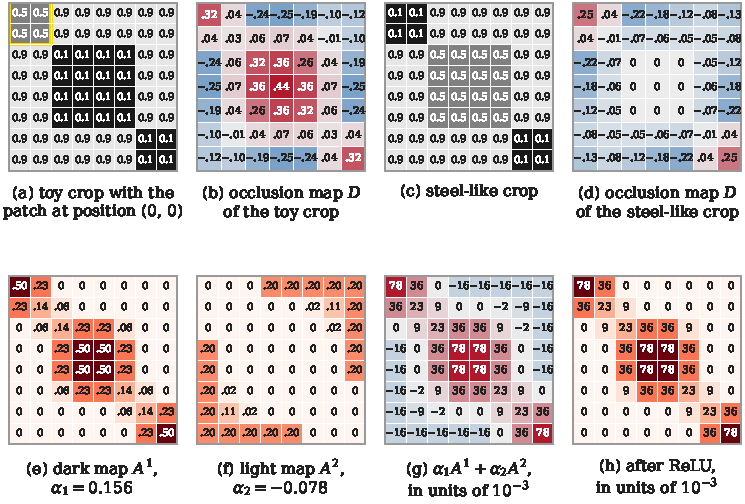
\includegraphics[width=\textwidth]{ch3_figures/fig_ch3_methods_toy.pdf}
\caption[Occlusion sensitivity and Grad-CAM on the toy crop]{Occlusion sensitivity and
Gradient-weighted Class Activation Mapping (Grad-CAM) on the toy crop. (a) Tight crop
with the grey $2 \times 2$ patch at position $(0, 0)$; (b) occlusion map $D$, drop of the
logit per patch position, (blue) negative, (red) positive; (c) steel-like crop,
workpiece at the fill value 0.5; (d) its occlusion map; (e) dark and (f) light feature
map with the Grad-CAM weights $\alpha_1$ and $\alpha_2$; (g) weighted sum of the feature
maps and (h) Grad-CAM map after the rectified linear unit (ReLU), both in units of
$10^{-3}$.}
\label{fig:bg-methods-toy}
\end{figure}

% ============================================================================
\subsection{Grad-CAM}
\label{sec:background-gradcam}

\paragraph{From CAM to Grad-CAM}
Class activation mapping (CAM)~\cite{zhou2016cam} applies to networks whose last feature
maps are globally averaged and fed into a single linear layer. The map of a class is
then the sum of the feature maps, each weighted by its weight in that linear layer, and
shows where the channels that favour the class are active. Gradient-weighted Class
Activation Mapping (Grad-CAM)~\cite{selvaraju2017gradcam} drops this restriction on the
architecture by taking the weights from the gradient. For feature maps
$A^k \in \mathbb{R}_{\ge 0}^{U \times V}$, $k = 1, \dots, K$, of a chosen layer and the
target logit $z$, the weight of channel $k$ is the mean gradient over its map,

\begin{equation}
\alpha_k = \frac{1}{UV} \sum_{u=0}^{U-1} \sum_{v=0}^{V-1}
\frac{\partial z}{\partial A^k_{uv}},
\label{eq:bg-gradcam-weights}
\end{equation}

where $\alpha_k \in \mathbb{R}$ and $U \times V$ is the size of the map. With the weights
of Eq.~\eqref{eq:bg-gradcam-weights}, the Grad-CAM map is the positive part of the
weighted sum of the maps,

\begin{equation}
G = \mathrm{ReLU}\Big( \sum_{k=1}^{K} \alpha_k A^k \Big),
\label{eq:bg-gradcam-map}
\end{equation}

where the ReLU acts element by element and $G \in \mathbb{R}_{\ge 0}^{U \times V}$. A
positive $\alpha_k$ marks a channel whose activity raises the logit on average over the
map, and the ReLU keeps
only the places where such channels outweigh the others. For display and comparison,
$G$ is divided by its maximum. If the weighted sum has no positive entry, $G$ is zero
everywhere and cannot be scaled. How often this happened in the thesis is reported in
Section~\ref{sec:results-degeneracy}. The map has the resolution of the layer it is
attached to. For c4 this is $32 \times 32$, i.e., one cell per 8 pixels of the
$256 \times 256$ input.

\paragraph{Grad-CAM on the toy}
In the toy, Eq.~\eqref{eq:bg-chain} already gives the gradient. The dark map has 16
cells with $10/16$ and 48 with zero, so its mean is
$\alpha_1 = 10/64 = +0.156$. The light map has the factor $-5$ instead of 10, so
$\alpha_2 = -5/64 = -0.078$ (Fig.~\ref{fig:bg-methods-toy}\,(e) and~(f)). The weighted
sum of Fig.~\ref{fig:bg-methods-toy}\,(g) is negative on the light background ring along
the crop border, $-0.078 \cdot 0.20 = -0.016$, and the ReLU sets it to zero
(Fig.~\ref{fig:bg-methods-toy}\,(h)). The map peaks at $0.156 \cdot 0.50 = 0.078$ at the
centre of the workpiece, and equally at the two factory parts. Grad-CAM thus marks every
place where the positively weighted dark channel is active, whether that place is the
workpiece or not. Because the toy has no pooling before its feature maps, the map has
the full $8 \times 8$ resolution of the input.

\paragraph{Where, not what}
Grad-CAM shows where channels with a positive weight are active, not what kind of
feature these channels respond to. A channel that responds to dark regions and one that
responds to a surface texture can look the same in $G$. For aluminium, Grad-CAM places
the evidence on the workpiece at most ratios (Section~\ref{sec:related-work-o2i}), but
the map cannot tell whether the model uses the shape of the workpiece or the texture of
its reflecting surface, the distinction that Geirhos et al.~\cite{geirhos2019texture}
draw for ImageNet-trained CNNs.

\paragraph{Grad-CAM on a real crop}
Fig.~\ref{fig:bg-methods-real}\,(d) shows two of the 256 feature maps of c4 for the crop
at 70\%, $A^{61}$ with $\alpha_{61} = +2.7 \times 10^{-5}$ and $A^{78}$ with
$\alpha_{78} = -4.3 \times 10^{-4}$, the channels that add most to and subtract most from
the weighted sum. Both respond mainly to the red plate around the workpiece and hardly to
the workpiece itself, one with a small positive and the other with a negative weight. Of
the 256 weights, 128 are positive and 128 negative, so the map of
Eq.~\eqref{eq:bg-gradcam-map} is a balance of many channels that push the logit in
opposite directions. The measured $32 \times 32$ map of
Fig.~\ref{fig:bg-methods-real}\,(e) covers the centre and the lower front of the
workpiece, and it marks the dark band along the top edge of the crop, outside the
reference square, only weakly. This is
one image and is meant as an illustration. How the Grad-CAM evidence spreads at 30\% and
10\% is shown in Section~\ref{sec:results-qualitative}. In contrast to occlusion, which
needed 225 separate local tests for the map of panel (b), Grad-CAM reads all feature
maps at once in one forward and one backward pass.

\begin{figure}[tbp]
\centering
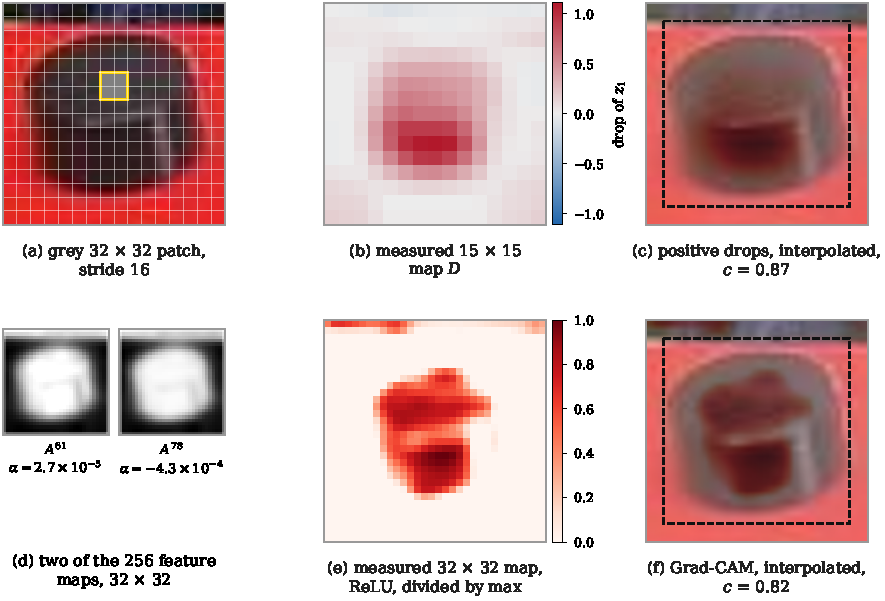
\includegraphics[width=\textwidth]{ch3_figures/fig_ch3_methods_real.pdf}
\caption[Occlusion sensitivity and Grad-CAM on one real crop]{Occlusion sensitivity and
Gradient-weighted Class Activation Mapping (Grad-CAM) for one crop of black plastic at
an object-to-image (O2I) ratio of 70\% (photograph 2024-04-15-095336) and the 70\%
black-plastic model. (a) Crop with one grey $32 \times 32$ patch and the stride-16 grid;
(b) measured $15 \times 15$ map $D$ of drops of the positive-class logit $z_1$;
(c) positive drops, normalised and bilinearly interpolated for display, with the
reference square (dashed) and the centre measure $c$; (d) two of the 256 feature maps
of the fourth convolutional layer, $32 \times 32$, with their weights $\alpha$ (dark
for high activation);
(e) measured $32 \times 32$ Grad-CAM map after the rectified linear unit (ReLU),
divided by its maximum; (f) Grad-CAM, interpolated for display, with $c$. The smooth
appearance of (c) and (f) comes from the interpolation, not from the measurement.}
\label{fig:bg-methods-real}
\end{figure}

% ============================================================================
\subsection{Object versus Background in a Heatmap}
\label{sec:background-comparison}

The research question asks whether the evidence of a model lies on the workpiece or on
the background. For one heatmap, this becomes the question whether the map favours the
workpiece. Since every crop is centred on its box, the workpiece is approximated by a
centred reference square with the area of the box, the dashed square in
Fig.~\ref{fig:bg-o2i}\,(d). Two summaries of a map suggest themselves. The first is the
share of the summed map that lies inside the square. The second compares the mean
importance per pixel inside the square with that outside it.

\paragraph{Why per pixel}
Fig.~\ref{fig:bg-centre-toy} applies both summaries to the toy. A flat map, with the same
value everywhere, has no preference for either region. Its share inside the square
equals the area of the square, 0.25 for the tight crop and 0.06 for the loose one
(panels (a) and (b)), so the share of a map without any preference changes with the
ratio. Its mean per pixel is the same inside and outside, and the per-pixel comparison
gives 0.50 for any square. Only the per-pixel version thus has a fixed level for ``no
preference''. This thesis therefore uses the per-pixel comparison and calls it the
centre measure $c$. It is defined exactly in Eq.~\eqref{eq:center-frac}
(Section~\ref{sec:methodology-centerfrac}). Values above 0.5 mean that a pixel inside the
square carries more importance on average than a pixel outside it, and values below 0.5
the reverse.

The toy maps of panels (c) and (d) both favour the workpiece. For occlusion, only the
positive drops are kept, each pixel receives the mean of the positive drops of the
patches that cover it, and the map is divided by its maximum. This gives $c = 0.83$. The Grad-CAM map divided by its
maximum gives $c = 0.84$. A pixel inside the square is thus about 4.9 and 5.2 times as
important as a pixel outside it. The shares of 0.62 and 0.64 are lower, because the
square covers only a quarter of the crop. For the real crop of
Fig.~\ref{fig:bg-methods-real}, $c$ is 0.87 for the positive occlusion drops and 0.82 for
Grad-CAM. The slightly lower Grad-CAM value seems to come from its weak response along
the dark band at the top edge, which lies outside the square. At this ratio, however, no occlusion patch lies
entirely outside the square, so the two values are not fully comparable
(Section~\ref{sec:methodology-resolution}).

\begin{figure}[tbp]
\centering
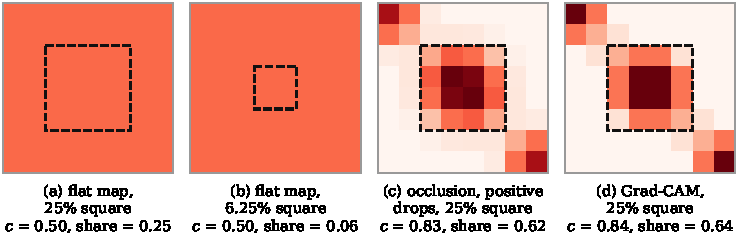
\includegraphics[width=\textwidth]{ch3_figures/fig_ch3_centre_measure_toy.pdf}
\caption[Comparing importance inside and outside a centred square on the
toy]{Comparing importance inside and outside a centred square on the toy, where $c$ is
the centre measure and share is the part of the summed map inside the square (dashed).
(a, b) Flat map with the square of the tight and of the loose crop; (c) occlusion map
with positive drops only, each pixel the mean of the positive drops of the patches that
cover it, divided by its maximum; (d) Grad-CAM map divided by its maximum, where Grad-CAM stands for
Gradient-weighted Class Activation Mapping.}
\label{fig:bg-centre-toy}
\end{figure}

\paragraph{Why the two methods can disagree}
Occlusion and Grad-CAM answer different questions. Occlusion asks what replacing one
patch with grey changes in the score while the rest of the image stays in place.
Grad-CAM asks where the channels that push the score up are active. Both can be right
about their own question and still point to different regions, and neither map is
ground truth for what the model uses~\textbf{[CITATION NEEDED]}. One way in which the
two answers could separate is a hypothesis that this thesis cannot test directly. If the
background contains many similar cues, like a room full of clocks, covering one of them
leaves the others visible and changes the score little, while Grad-CAM marks all of
them at once.

The toy does not show such a divergence. Its two maps agree, with $c = 0.83$ and 0.84.
What it shows are the ingredients. Both methods mark the dark factory parts, but for
different reasons: Grad-CAM because the dark channel is active there, occlusion because
covering them lowers the score. In the toy the two reasons coincide, but nothing forces
them to. Occlusion also depends on the fill, and for the steel-like crop it
places all positive evidence outside the workpiece. Its drops can be negative, so the
treatment of negative values enters the summary.

Other questions the toy cannot settle at all. Its patch is chosen to fit its workpiece,
its maps are read without interpolation, and its square is exactly the workpiece. The
real crops have none of these conveniences: 75 models at five ratios, patches on a
$256 \times 256$ input, coarse maps that must be brought to the pixel grid, and a
square that only approximates a box that itself encloses some background. Before values
of $c$ can be compared across materials and ratios, each of these needs a fixed and
justified setting, and Section~\ref{sec:methodology} provides them.
